% Здесь пишется содержание первой главы
%
\chapter{\MakeUppercase{Разведочный анализ данных с использованием PySpark}}\label{ch:first}
\section{Постановка задачи разведочного анализа}\vspace{\baselineskip}

Здесь нужно сформулировать постановку задачи разведочного анализа: что дано, и что нужно сделать.

\vspace{\baselineskip}\section{Описание датасета}\vspace{\baselineskip}

Здесь требуется описать выбранный датасет, привести ссылку на него, охарактеризовать его тематику, объем, количество признаков. Вкратце нужно описать признаки датасета (допускается описывать не все признаки, а только те, которые используются в исследовании).
Также, можно сослаться на источники, например, в \cite{karau2015spark, koirala2020pyspark, white2013hadoop, Tekdogan2022} рассматривается материал об ... Часть информации можно оформить в виде таблицы, но избегайте слишком длинных таблиц. На каждую таблицу должна быть ссылка в тексте, как, например, на таблицу \ref{tab:features}, в которой приведен пример описания признаков.

\begin{table}[]
    \centering
    \begin{tabularx}{\textwidth}{|X|X|}
        \hline
        \multicolumn{1}{|c|}{Признак}  & \multicolumn{1}{c|}{Расшифровка признака}   \\ \hhline{|=|=|}
        Temperature                    & Среднемесячная температура в \degree C      \\ \hline
        Humidity                       & Влажность в процентах                       \\ \hline
    \end{tabularx}
    \caption{Пример таблицы признаков}
    \label{tab:features}
\end{table}

\vspace{\baselineskip}\section{Определение пропущенных значений}\vspace{\baselineskip}

Обратите внимание, что приведенная здесь структура раздела не является жестким требованием, а служит примером оформления. При необходимости, её можно корректировать в разумных пределах.

При необходимости можно вставить рисунок и сослаться на него: на рисунке \ref{fig:HadoopEcoSystem} приведена иллюстрация экосистемы Hadoop. Обратите внимание, что таблицы и рисунки являются <<плавающими>> объектами: они могут располагаться не в месте их непосредственного объявления, а в некоторой близости от него.

\begin{figure}
    \centering
    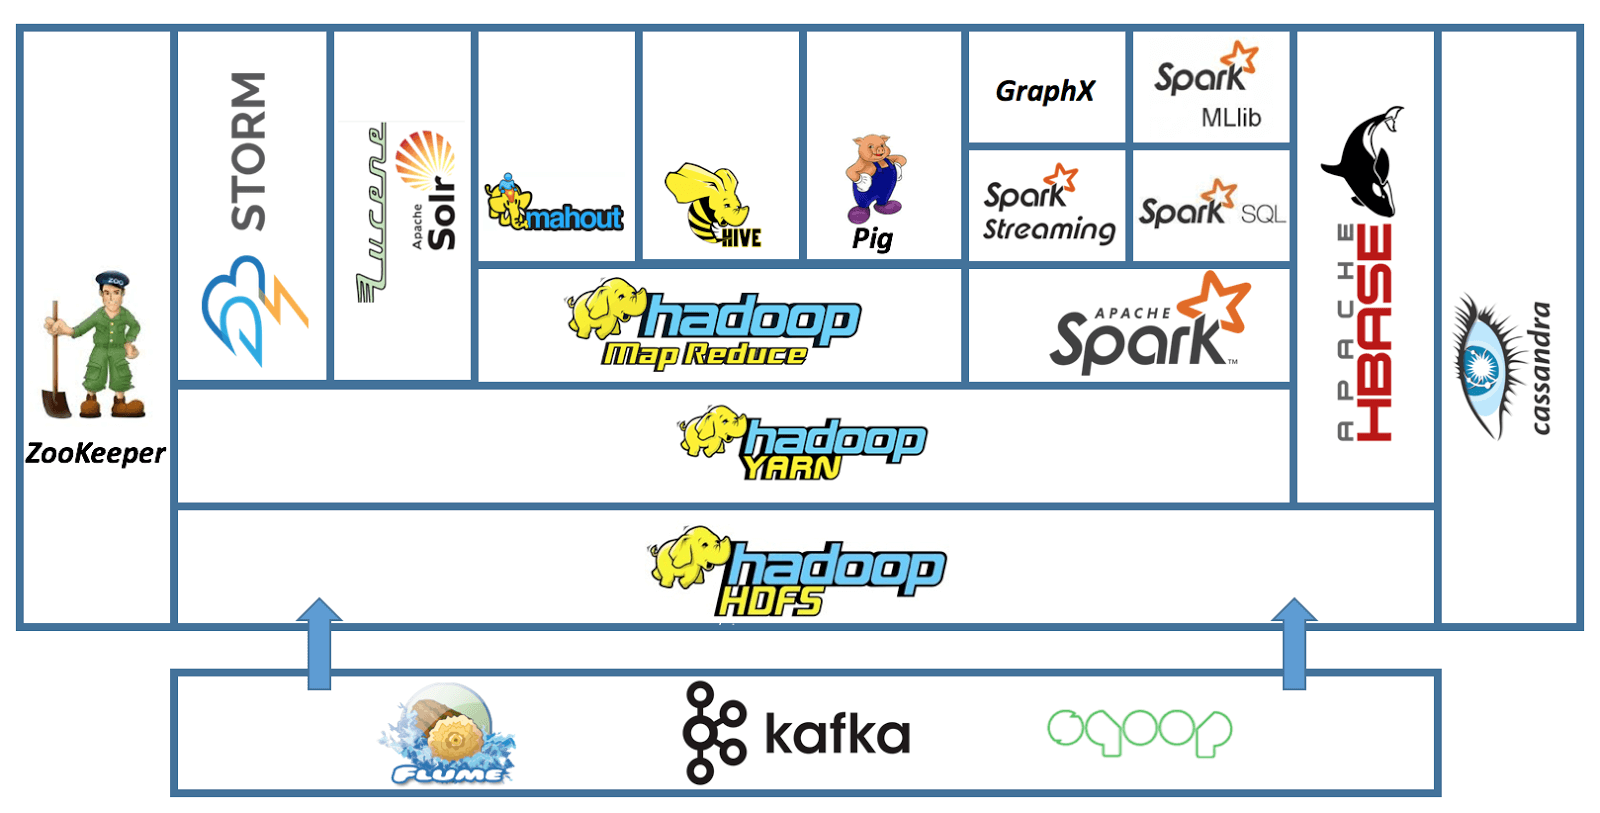
\includegraphics[width=\textwidth]{Content/Images/HadoopEcoSystem.png}
    \caption{Иллюстрация экосистемы Hadoop}
    \label{fig:HadoopEcoSystem}
\end{figure}

Также, вот пример списка:

\begin{itemize}
    \item первый элемент;
    \item второй элемент;
    \item третий элемент;
    \begin{itemize}
        \item вложенный элемент.
    \end{itemize}
\end{itemize}

А здесь -- аналогичный нумерованный список:

\begin{enumerate}
    \item первый элемент;
    \item второй элемент;
    \item третий элемент;
    \begin{enumerate}
        \item вложенный элемент.
    \end{enumerate}
\end{enumerate}

А вот формула, которая связывает между собой синус, косинус и тангенс.

\begin{equation}
    \label{eq:formula}
    \tg \alpha = \frac{\sin \alpha}{\cos \alpha}.
\end{equation}

Ну, и ссылка на неё: формула (\ref{eq:formula}) выражает связь тригонометрических функций.

\vspace{\baselineskip}\section{Другая подглава}\vspace{\baselineskip}

Здесь можно продемонстрировать пример включения фрагмента кода в текст работы. И заодно добавить еще пару ссылок \cite{spark2022official, zaharia2021lakehouse}.
\begin{code}
import matplotlib.pyplot as plt
import numpy as np
x = np.linspace(0, 10, 100)
y = np.sin(x)
plt.figure(figsize=(10, 6))
plt.plot(x, y, label='sin(x)', color='blue', linewidth=2)
plt.title('График функции sin(x)', fontsize=16)
plt.xlabel('x', fontsize=14)
plt.ylabel('sin(x)', fontsize=14)
plt.legend()
plt.grid(True)
plt.show()    
\end{code}

Здесь продолжается текст. Не забывайте, что фрагмент кода не должен превышать половины страницы -- затем должен следовать текст.

\vspace{\baselineskip}\section{Выводы}\vspace{\baselineskip}

В конце каждой главы должны быть выводы. Они представляют собой несколько предложений, которые кратко характеризуют проделанную в главе работу и полученные результаты.
